\documentclass[a4paper,12pt]{article}

\author{\textbf{Софиа Белен Лопес Висенс}\\
    Группа Б02-903\\ 
\large Московский физико-технический институт}
\title{\textbf{Задание 2}\\
Молекурялная динамика}
\date{}

\usepackage[margin=0.9in]{geometry}
\usepackage{graphicx}
\usepackage{float}
\usepackage[utf8]{inputenc}
\usepackage[T2A]{fontenc}
\usepackage{textcomp}
\usepackage{amsmath, amssymb}
\usepackage{siunitx}
\usepackage{subcaption}
\usepackage{multirow}
\usepackage{xcolor}

\definecolor{grey}{HTML}{ba000f}
\definecolor{red}{HTML}{990505}
\definecolor{green}{HTML}{2e8a07}

\renewcommand{\figurename}{Рис.}
\renewcommand{\tablename}{Таблица}
\renewcommand*\contentsname{Содержание}

\begin{document}
\maketitle
\newpage
\tableofcontents
\newpage

\section{Радиальная функция распределения}

\begin{figure}[H]
    \centering
    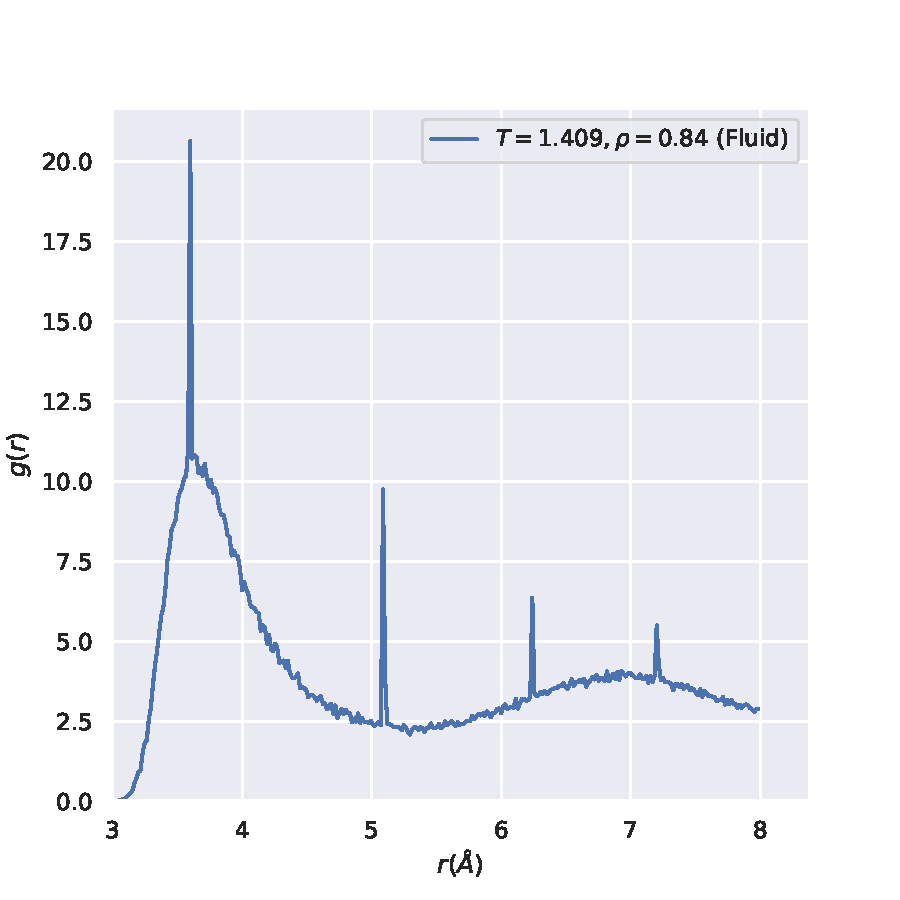
\includegraphics[width=0.8\textwidth]{../../media/rdfYarnell.pdf}
\caption{Радиальная функция распределения для жидкого Аргона
при \(\rho = 0.0213 \frac{atoms}{\si{\angstrom}^3}\), 
\(T = 85^\circ K\). Соответственные параметры в единицах
Леннарда-Джонса \(\rho = 0.84\), \(T = 1.409\).}
\end{figure}

\section{Автокорреляционная функция скорости}

\begin{figure}[H]
    \centering
    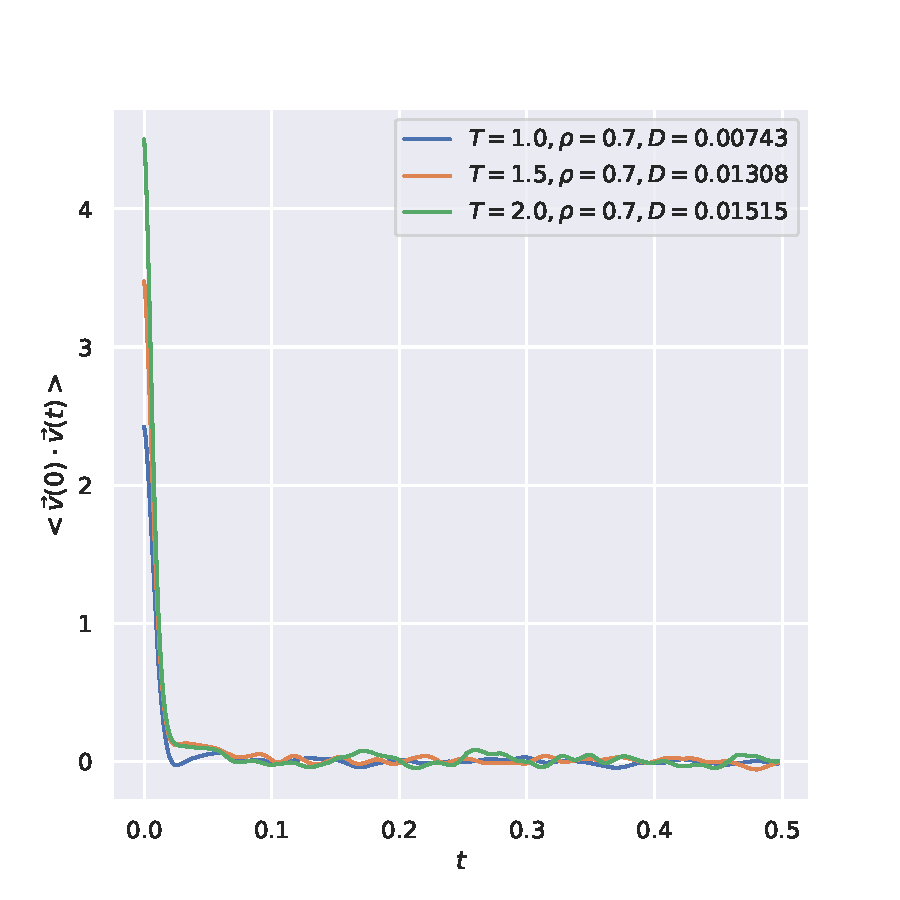
\includegraphics[width=0.8\textwidth]{../../media/vac.pdf}
\caption{График автокорреляционной функции
    скорости в зависимости от времени при различных
температурах. Расчёт коэффициент самодиффузии с
помощью формулы Грина-Кубо.}
\end{figure}

\section{Расчёт коэффициента самодиффузии}

{\color{red} Maybe we are still in subdiffusive regime?
But then shouldn't D be lower than expected, and not
higher? That probably means we are still in ballictic
regime.}

\begin{figure}[H]
    \centering
    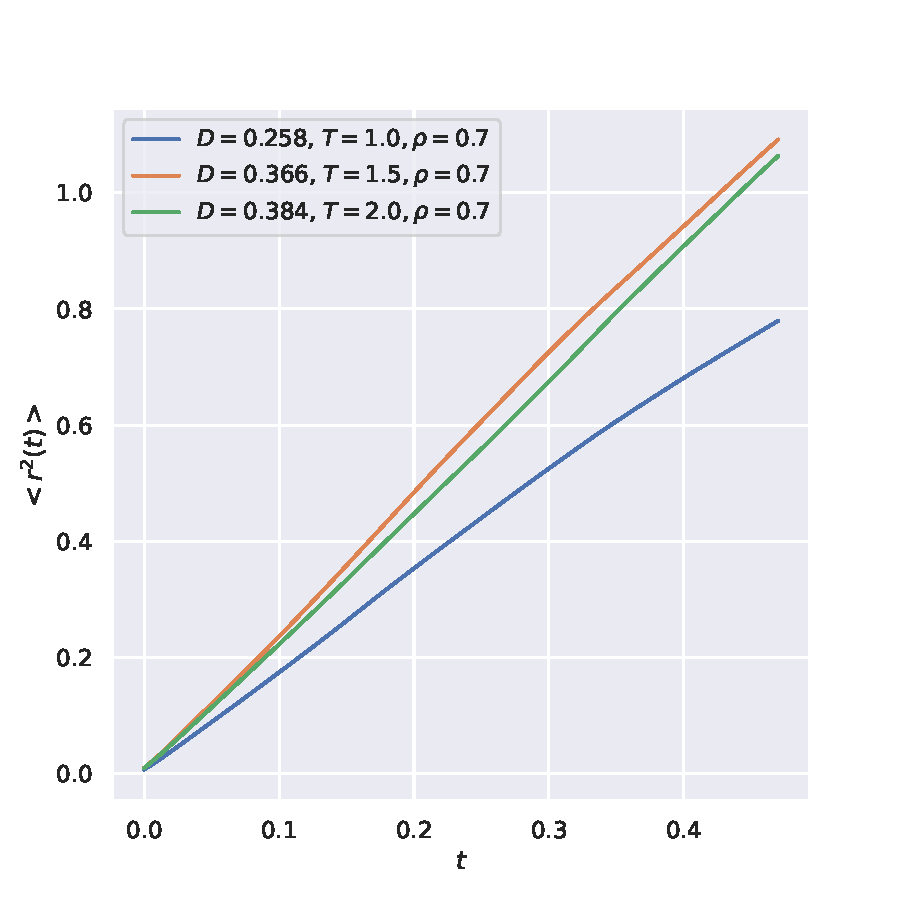
\includegraphics[width=0.8\textwidth]{../../media/diffusion.pdf}
\caption{График зависимость среднего квадратичного
смещения в зависимости от времени. Расчет коэффициента
самодиффузии через формулу Эйнштейна-Смолуховского.}
\end{figure}

\begin{table}[H]
    \centering
    \caption{Коэффициент самодиффузии полученный через
    формулу Эйнштейна-Смолуховского и Грина-Кубо при 
\(\rho = 0.7\).}
    \label{tab:label}
    \begin{tabular}{|c | c | c | c |}
        \hline
        Темература & Эйнштейна-Смолуховского & Грина-Кубо 
                   & Ожидаемое значение\\
        \hline
        \hline
        1.0 & 0.258 & 0.00743 & {\color{red}0.105} \\
        1.5 & 0.366 & 0.01308 & {\color{red}0.156} \\
        2.0 & 0.384 & 0.01515 & {\color{red}0.217} \\
        \hline
    \end{tabular}
\end{table}

\section{Сравнение с первым заданием}

{\color{red} Вопрос: Как это \(<\Delta r^2(t)>\)
связано с значением из другого пункта?}

\begin{figure}[H]
    \centering
    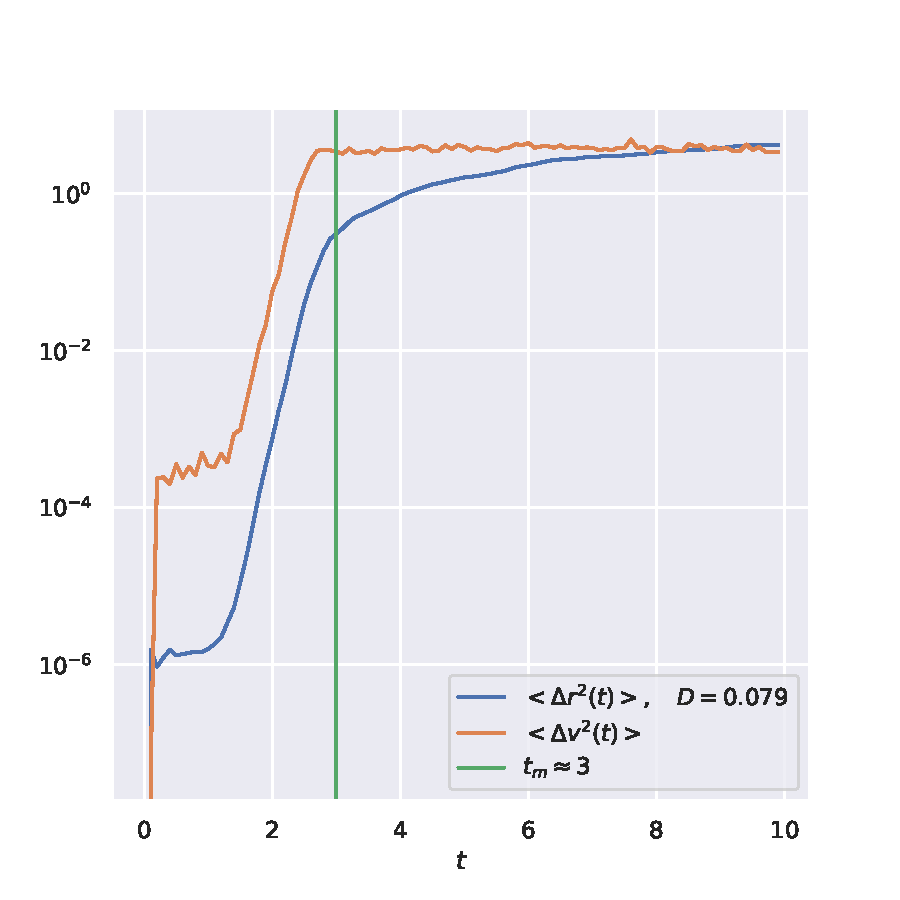
\includegraphics[width=0.8\textwidth]{../../media/tm.pdf}
\caption{Усреднённые разбегания координат \(<\Delta r^2(t)>\) 
и скоростей \(<\Delta v^2(t)>\) на двух траекториях,
рассчитанных из тождественных начальных условий с 
шагами \(\Delta t_1 = 0.001\) и \(\Delta t_2 = 0.0001\).
При температуре \(T = 1.0\) и плотности 
\(\rho = 0.7\) получим коэффициент
самодиффузии \(D = 0.079\). Он оказывается на порядок
меньше значения полученного с помощью соотношения
Эйнштейна-Смолуховского}
\end{figure}

\section{Влияние термостата на расчет коэффициента диффузии}

\begin{figure}[H]
    \centering
    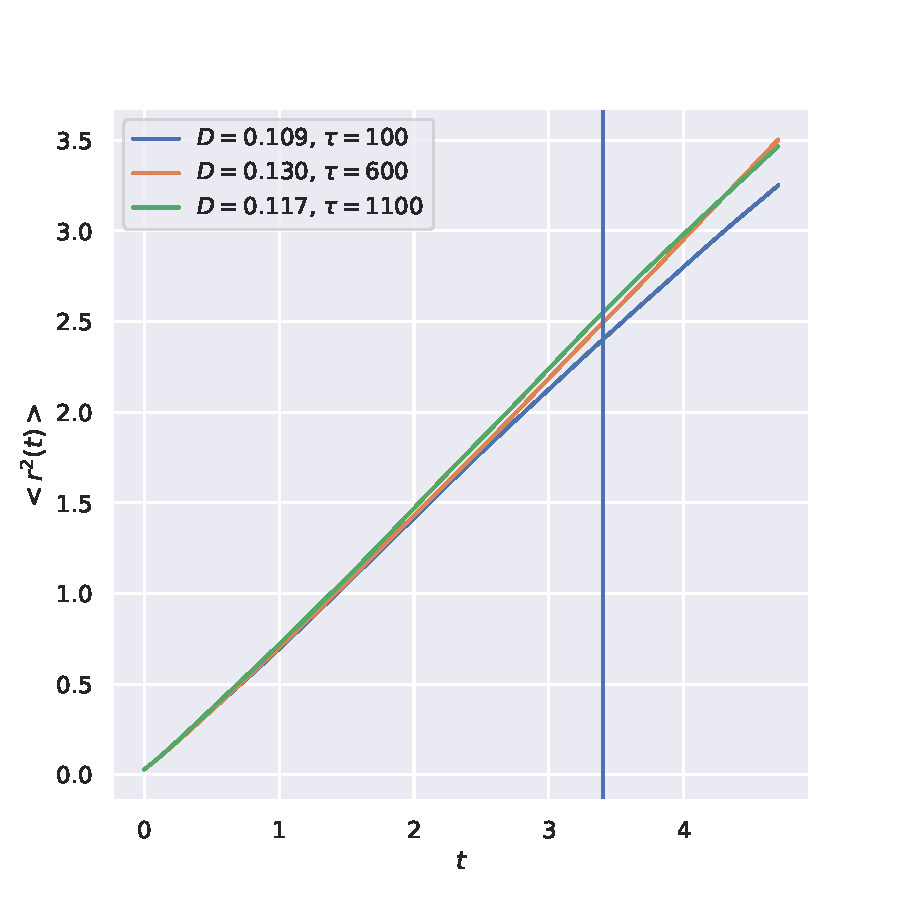
\includegraphics[width=0.8\textwidth]{../../media/thermostat.pdf}
\caption{График зависимость среднего квадратичного
смещения в зависимости от времени. Расчет коэффициента
самодиффузии через формулу Эйнштейна-Смолуховского при
температуре \(T = 1.5\) для различных характерных 
величин термостата \(\tau\).
Вертикальная линия момент, начиная с которого 
мы рассчитаем коэффициент диффузии.}
\end{figure}

\end{document}

